\chapter{Piles, piles à combustible et électrolyse}\label{ch:b2:batteries-electrolysis}

Chaque kilogramme d'aluminium extrait de son minerai exige environ \qty{13}{kW.h}
d'électricité~; refondre un kilogramme de déchets exige, en principe, les
\qty{0.3}{kW.h} qui le portent à sa température de fusion et le fondent. La différence
est le travail d'une longue rangée de cuves d'\omterm{def:b2:batteries-electrolysis:electrolysis}{électrolyse}, chacune faisant passer des centaines de
milliers d'ampères dans un sel fondu sous quelques volts. Une pile fonctionne dans
l'autre sens~: une réaction spontanée entraîne le courant. Grâce aux
\omterm{def:b2:current-potential-curves:ie-curve}{courbes intensité--potentiel} du \cref{ch:b2:current-potential-curves}, les deux se
lisent sur le même diagramme, de même qu'un morceau de zinc qui se dissout dans un acide.
% ledger: hT:Al_l.933, aw:Al

\begin{recall}
\Cref{ch:b2:cell-thermodynamics}~: $\Delta_r G = -nFE$, travail maximal, \omterm{def:b2:cell-thermodynamics:faraday}{constante
de Faraday}. \Cref{ch:b2:current-potential-curves}~: \omterm{def:b2:current-potential-curves:ie-curve}{courbes intensité--potentiel},
\omterm{def:b2:current-potential-curves:fast-slow}{systèmes rapides} et lents, \omterm{def:b2:current-potential-curves:overpotential}{surtensions}, \omterm{def:b2:current-potential-curves:limiting-current}{courants limites}, murs de
l'eau. \Cref{ch:b2:ellingham}~: pourquoi l'aluminium ne s'obtient pas par le carbone. Le volume
scolaire~: \omterm{def:b2:batteries-electrolysis:electrolysis}{électrolyse}, \omterm{def:b2:batteries-electrolysis:battery}{accumulateurs}.
\end{recall}

\begin{omfigure}
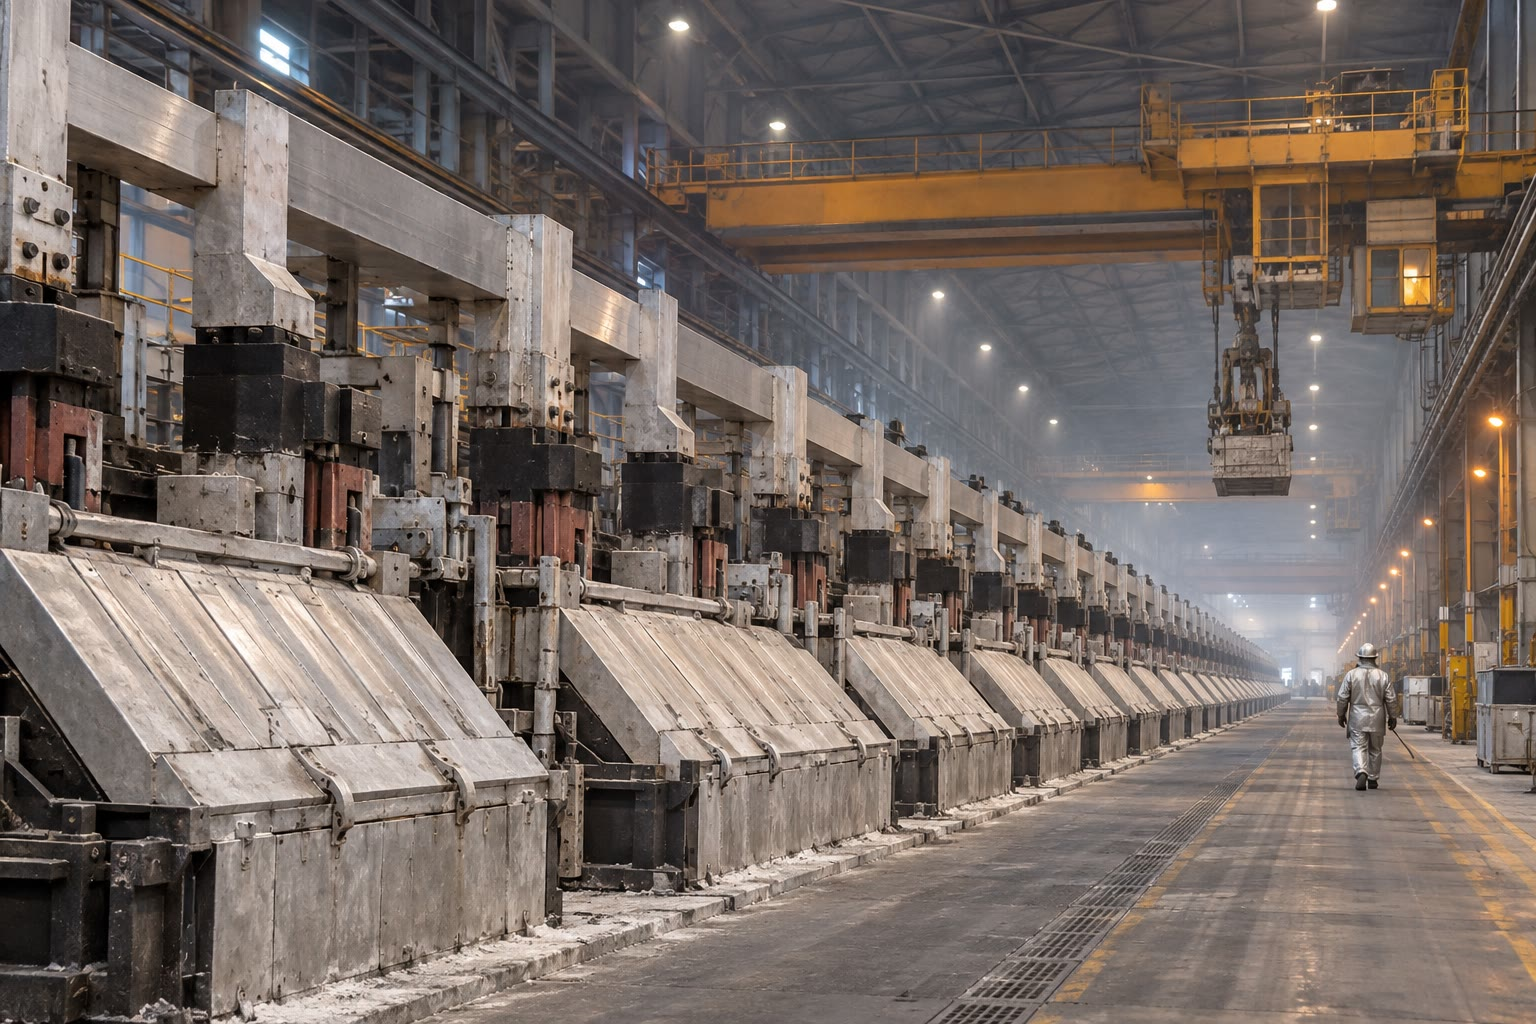
\includegraphics[width=0.62\linewidth]{images/book3/ai/b2-11-potroom.jpg}

{\small La halle d'\omterm{def:b2:batteries-electrolysis:electrolysis}{électrolyse} d'une aluminerie~: une rangée de cuves d'\omterm{def:b2:batteries-electrolysis:electrolysis}{électrolyse},
longue de plusieurs centaines, montées en série~; le pont roulant remplace les anodes
de carbone à mesure qu'elles brûlent.}
\end{omfigure}

\section{Les réactions spontanées lues sur les courbes}

\begin{definition}[Potentiel mixte]\label{def:b2:batteries-electrolysis:mixed-potential}
Le \emph{potentiel mixte}\index{potentiel mixte} d'une électrode sur laquelle réagissent deux
couples différents, l'un oxydé et l'autre réduit, est le potentiel qu'elle
prend lorsqu'aucun courant net ne la traverse~: le \omterm{def:b2:current-potential-curves:ie-curve}{courant anodique} d'un couple est alors
égal et opposé au \omterm{def:b2:current-potential-curves:ie-curve}{courant cathodique} de l'autre.
\end{definition}

\begin{proposition}[Un métal dans une solution]\label{prop:b2:batteries-electrolysis:mixed}
Un métal plongé dans une solution capable de l'oxyder se fixe au potentiel
$E_m$ tel que $i_a(E_m) = -i_c(E_m)$, le \omterm{def:b2:current-potential-curves:ie-curve}{courant anodique} d'oxydation du métal
compensant le \omterm{def:b2:current-potential-curves:ie-curve}{courant cathodique} de réduction de l'oxydant~; le
métal se dissout à la vitesse $i_a(E_m)/(nF)$.
\end{proposition}

\begin{proof}
Un morceau de métal isolé ne porte aucun courant net. Les deux demi-réactions ont lieu
à sa surface au même potentiel~: leurs courants, lus sur leurs courbes
à ce potentiel, ont donc une somme nulle. D'après la \cref{prop:b2:current-potential-curves:current-rate},
le \omterm{def:b2:current-potential-curves:ie-curve}{courant anodique} donne la vitesse d'oxydation.
\end{proof}

\begin{omfigure}
\begin{tikzpicture}
\begin{axis}[omie, width=0.82\linewidth, height=6cm, xmin=-1.1, xmax=-0.3,
  ymin=-3, ymax=3, xlabel={$E$ (V)}, ylabel={$i$}, clip=true, clip mode=individual,
  axis y line=left]
\addplot[omanodic] table[x=E, y=i] {figdata/out/bachelor-2-ie-curves-f-Zn.dat};
\addplot[omcathodic] table[x=E, y=i] {figdata/out/bachelor-2-ie-curves-f-HZn.dat};
\addplot[omcathodic, dashed] table[x=E, y=i] {figdata/out/bachelor-2-ie-curves-f-HCu.dat};
\draw[densely dotted] (axis cs:-0.820,-0.148) -- (axis cs:-0.820,0.148);
\draw[densely dotted] (axis cs:-0.737,-2.38) -- (axis cs:-0.737,2.38);
\fill (axis cs:-0.820,0.148) circle (1.3pt); \fill (axis cs:-0.737,2.38) circle (1.3pt);
\node[font=\scriptsize, anchor=south east] at (axis cs:-0.825,0.2) {zinc seul};
\node[font=\scriptsize, anchor=west] at (axis cs:-0.73,2.38) {zinc au contact du cuivre};
\node[font=\scriptsize, omThm, anchor=west] at (axis cs:-0.70,1.2) {\ce{Zn} $\to$ \ce{Zn^2+}};
\node[font=\scriptsize, omDef, anchor=north west, align=left] at (axis cs:-0.87,-0.5) {\ce{H+} $\to$ \ce{H2}\\ sur zinc};
\node[font=\scriptsize, omDef, anchor=north west] at (axis cs:-0.66,-1.7) {sur cuivre};
\end{axis}
\end{tikzpicture}

{\small Zinc dans un acide (courbes modèles, ions zinc dilués~; potentiels de
$-1.1$ à \qty{-0.3}{V}). Seul, le zinc se fixe au
\omterm{def:b2:batteries-electrolysis:mixed-potential}{potentiel mixte} où son oxydation compense la réduction lente de
\ce{H+} sur le zinc~: un courant faible, une dissolution lente. Au contact du cuivre, sur lequel
la réduction de \ce{H+} est moins lente, l'équilibre se déplace vers un potentiel plus élevé
et un courant plus de dix fois plus grand~: le zinc se dissout vite, du dihydrogène
se dégage sur le cuivre.}
\end{omfigure}

La même lecture explique la corrosion (\cref{ch:b2:corrosion})~: la vitesse de corrosion
d'un métal est le courant à son \omterm{def:b2:batteries-electrolysis:mixed-potential}{potentiel mixte}.

\section{Les piles qui débitent un courant}

\begin{definition}[Piles et accumulateurs]\label{def:b2:batteries-electrolysis:battery}
Une \emph{pile primaire}\index{pile primaire} est une cellule électrochimique utilisée
une seule fois, jusqu'à épuisement de ses réactifs. Un \emph{accumulateur}\index{accumulateur}
est une cellule que l'on peut recharger en la faisant traverser par un courant de
sens inverse, qui inverse sa réaction. L'\emph{énergie
massique}\index{energie massique@énergie massique} d'une cellule est l'énergie électrique qu'elle fournit
par unité de masse, en général en \unit{W.h/kg}.
\end{definition}

\begin{proposition}[Tension d'une pile qui débite un courant]\label{prop:b2:batteries-electrolysis:delivering}
Une pile qui débite un courant $I$ a pour tension
\[
  U = E_+ - E_- - \eta_a - |\eta_c| - rI ,
\]
où $E_+$ et $E_-$ sont les potentiels d'équilibre de ses deux électrodes,
$\eta_a > 0$ la \omterm{def:b2:current-potential-curves:overpotential}{surtension} de l'oxydation à l'électrode négative,
$\eta_c < 0$ celle de la réduction à l'électrode positive, et $r$ la
résistance interne (électrolyte, séparateur, connexions).
\end{proposition}

\begin{proof}
Le même courant $I$ est anodique à l'électrode négative, dont le potentiel se
lit sur sa courbe anodique, $E_- + \eta_a$, et cathodique à l'électrode positive,
dont le potentiel vaut $E_+ + \eta_c$. Entre elles, le courant traverse
l'électrolyte, où le potentiel chute de $rI$. D'où $U = (E_+ + \eta_c) - (E_- +
\eta_a) - rI$.
\end{proof}

\begin{omfigure}
\begin{tikzpicture}
\begin{axis}[omie, width=0.82\linewidth, height=5.6cm, xmin=-1.2, xmax=0.8,
  ymin=-2, ymax=2, xlabel={$E$ (V)}, ylabel={$i$}, clip=true, clip mode=individual]
\addplot[omanodic] table[x=E, y=i] {figdata/out/bachelor-2-ie-curves-h-neg.dat};
\addplot[omcathodic] table[x=E, y=i] {figdata/out/bachelor-2-ie-curves-h-pos.dat};
\draw[densely dashed, gray] (axis cs:-1.2,1) -- (axis cs:0.8,1);
\draw[densely dashed, gray] (axis cs:-1.2,-1) -- (axis cs:0.8,-1);
\node[font=\scriptsize, gray, anchor=south west] at (axis cs:-1.18,1) {$+I$};
\node[font=\scriptsize, gray, anchor=north west] at (axis cs:-1.18,-1) {$-I$};
\fill (axis cs:-0.730,1) circle (1.3pt); \fill (axis cs:0.210,-1) circle (1.3pt);
\draw[densely dotted] (axis cs:-0.85,0) -- (axis cs:-0.85,0.5);
\draw[densely dotted] (axis cs:0.45,0) -- (axis cs:0.45,-0.5);
\node[font=\scriptsize, anchor=south] at (axis cs:-0.85,0.5) {$E_-$};
\node[font=\scriptsize, anchor=north] at (axis cs:0.45,-0.5) {$E_+$};
\draw[<->, thick, omProp] (axis cs:-0.730,1.5) -- (axis cs:0.210,1.5) node[midway, above, font=\scriptsize] {$U + rI$};
\draw[densely dotted] (axis cs:-0.730,1) -- (axis cs:-0.730,1.5);
\draw[densely dotted] (axis cs:0.210,-1) -- (axis cs:0.210,1.5);
\node[font=\scriptsize, omThm, anchor=west] at (axis cs:-0.70,0.6) {électrode négative};
\node[font=\scriptsize, omDef, anchor=west] at (axis cs:0.30,-1.5) {électrode positive};
\end{axis}
\end{tikzpicture}

{\small Le point de fonctionnement d'une pile (courbes modèles). Sous un courant $I$,
l'électrode négative se trouve sur sa courbe anodique, l'électrode positive sur sa
courbe cathodique~; la différence des deux potentiels, diminuée de la chute ohmique
$rI$, est la tension délivrée. Elle diminue quand $I$ augmente.}
\end{omfigure}

\begin{method}[Le point de fonctionnement d'une pile ou d'un électrolyseur]\label{met:b2:batteries-electrolysis:operating-point}
\begin{enumerate}
  \item Tracer la courbe anodique de l'électrode qui est oxydée et la
        courbe cathodique de celle qui est réduite.
  \item Pour un courant $I$, lire le potentiel de chaque électrode en $+I$ sur la
        courbe anodique et en $-I$ sur la courbe cathodique.
  \item La différence des deux potentiels, corrigée de $rI$ (retranché pour
        une pile, ajouté pour un \omterm{def:b2:batteries-electrolysis:electrolysis}{électrolyseur}), est la tension.
\end{enumerate}
\end{method}

\begin{example}[L'accumulateur au plomb]\label{ex:b2:batteries-electrolysis:lead}
À l'électrode négative, \ce{Pb + SO4^2- -> PbSO4 + 2e-}~; à l'électrode positive,
\ce{PbO2 + 4H+ + SO4^2- + 2e- -> PbSO4 + 2H2O}. Au total,
\[
  \ce{Pb + PbO2 + 4H+ + 2SO4^2- -> 2PbSO4 + 2H2O},
\]
$\Delta_r G^\circ = 2(-813.14) + 2(-237.13) - (-217.33) - 2(-744.53) =
\qty{-394.1}{kJ/mol}$, $E^\circ = 394\,100/(2 \times 96\,485) = \qty{2.04}{V}$.
Les deux électrodes se couvrent de sulfate de plomb pendant la décharge~; la charge
inverse la réaction. La réduction de \ce{H+} sur le plomb et l'oxydation de
l'eau sur le dioxyde de plomb sont lentes~: c'est pourquoi un élément de \qty{2}{V} peut être chargé
dans l'eau, dont le domaine thermodynamique n'a que \qty{1.23}{V} de largeur.
% ledger: dfg:PbSO4_cr, dfg:H2O_l, dfg:PbO2_cr, dfg:SO42-_ao
\end{example}

\begin{omfigure}
\begin{tikzpicture}[font=\small, >={Stealth}]
  \draw[thick] (0,0) rectangle (6,3.2);
  \fill[omDef!10] (0.05,0.05) rectangle (5.95,2.7);
  \fill[black!45] (0.6,0.4) rectangle (1.1,2.9);
  \fill[brown!60!black] (4.9,0.4) rectangle (5.4,2.9);
  \draw[thick] (0.85,2.9) -- (0.85,3.9) node[pos=0.75, left] {$-$};
  \draw[thick] (5.15,2.9) -- (5.15,3.9) node[pos=0.75, right] {$+$};
  \draw[->, thick, omProp] (0.85,3.9) -- (0.85,4.3) -- (5.15,4.3) -- (5.15,3.95);
  \node[font=\scriptsize, omProp, anchor=south] at (3,4.3) {$\mathrm{e^-}$ à la décharge};
  \node[font=\scriptsize, align=center] at (0.85,-0.45) {\ce{Pb}\\ (\ce{PbSO4} à la décharge)};
  \node[font=\scriptsize, align=center] at (5.15,-0.45) {\ce{PbO2}\\ (\ce{PbSO4} à la décharge)};
  \node[font=\scriptsize, align=center] at (3.0,1.6) {solution de \ce{H2SO4}\\ \ce{H+}, \ce{HSO4-}, \ce{SO4^2-}};
\end{tikzpicture}

{\small L'\omterm{def:b2:batteries-electrolysis:battery}{accumulateur} au plomb, schéma. À la décharge, le plomb est oxydé
et le dioxyde de plomb réduit, tous deux en sulfate de plomb, et l'acide est consommé~: la
masse volumique de la solution indique l'état de charge.}
\end{omfigure}

\begin{omfigure}
\begin{tikzpicture}[font=\small, >={Stealth}]
  \draw[thick] (0,0) rectangle (7,3);
  % graphite layers
  \foreach \y in {0.5,0.9,1.3,1.7,2.1,2.5} \draw[thick, black!70] (0.3,\y) -- (2.3,\y);
  \foreach \y in {0.7,1.1,1.5,1.9,2.3} \foreach \x in {0.6,1.3,2.0} \fill[omDef] (\x,\y) circle (0.07);
  % layered oxide
  \foreach \y in {0.5,0.9,1.3,1.7,2.1,2.5} \draw[thick, omThm] (4.7,\y) -- (6.7,\y);
  \foreach \y in {0.7,1.5,2.3} \foreach \x in {5.0,5.7,6.4} \fill[omDef] (\x,\y) circle (0.07);
  \draw[densely dashed] (3.5,0) -- (3.5,3);
  \node[font=\scriptsize, align=center] at (1.3,-0.45) {graphite (négative)};
  \node[font=\scriptsize, align=center] at (5.7,-0.45) {oxyde lamellaire (positive)};
  \node[font=\scriptsize, anchor=south] at (3.5,3.0) {séparateur};
  \draw[->, thick, omThm] (2.5,2.1) -- (4.5,2.1) node[midway, above, font=\scriptsize, fill=white, inner sep=1pt] {\ce{Li+} à la décharge};
  \draw[<-, thick, omDef] (2.5,0.9) -- (4.5,0.9) node[midway, below, font=\scriptsize, fill=white, inner sep=1pt] {\ce{Li+} à la charge};
\end{tikzpicture}

{\small Un \omterm{def:b2:batteries-electrolysis:battery}{accumulateur} lithium-ion, schéma. Les ions lithium (points bleus) se logent entre les
feuillets du graphite dans l'\omterm{def:b2:batteries-electrolysis:battery}{accumulateur} chargé~; à la décharge, ils traversent
l'électrolyte pour s'insérer entre les feuillets d'un oxyde métallique, tandis que les électrons
parcourent le circuit extérieur. Aucune électrode n'est dissoute ni déposée~: les
ions font la navette entre deux structures d'accueil.}
\end{omfigure}

\begin{history}[La pile de Volta]
\begin{minipage}[t]{0.27\linewidth}
\vspace{0pt}
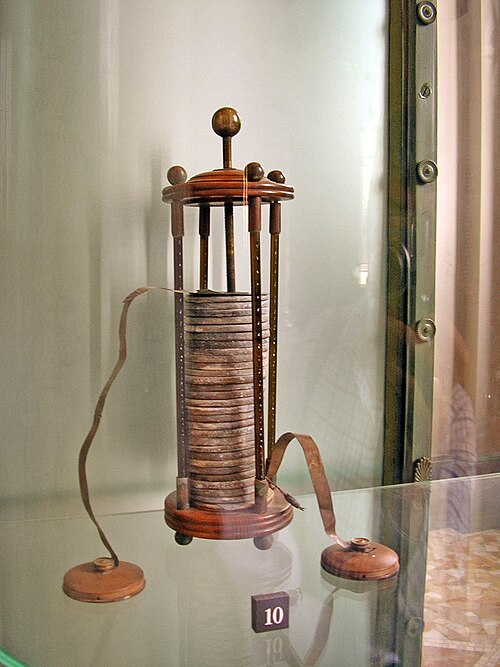
\includegraphics[width=\linewidth]{images/book3/volta-pile.jpg}
\end{minipage}\hfill
\begin{minipage}[t]{0.69\linewidth}
\vspace{0pt}
En 1800, Alessandro Volta décrivit une colonne de disques de deux métaux différents,
zinc et cuivre ou argent, séparés par des tissus imbibés de saumure~: la première
source de courant électrique continu. En quelques semaines, d'autres l'utilisèrent pour décomposer
l'eau, et en moins de dix ans Humphry Davy avait isolé le sodium et le potassium par
\omterm{def:b2:batteries-electrolysis:electrolysis}{électrolyse} de leurs hydroxydes fondus à l'aide d'une grande pile. La photographie montre
l'une des piles de Volta lui-même. (Photographie~: GuidoB, CC BY-SA 3.0, Wikimedia
Commons.)
\end{minipage}
\end{history}

\section{Les piles à combustible}

\begin{definition}[Pile à combustible]\label{def:b2:batteries-electrolysis:fuel-cell}
Une \emph{pile à combustible}\index{pile a combustible@pile à combustible} est une pile dont les réactifs, un combustible et un
oxydant (en général le dioxygène de l'air), sont apportés en continu à ses
électrodes et dont les produits sont évacués, de sorte qu'elle débite du courant tant
qu'elle est alimentée.
\end{definition}

Dans la pile à membrane échangeuse de protons du bus du
\cref{ch:b2:cell-thermodynamics}, le dihydrogène est oxydé sur un catalyseur au platine,
\ce{H2 -> 2H+ + 2e-}, les protons traversent une fine membrane polymère acide, et le dioxygène est
réduit de l'autre côté, \ce{O2 + 4H+ + 4e- -> 2H2O}. L'oxydation du dihydrogène
sur platine est un \omterm{def:b2:current-potential-curves:fast-slow}{système rapide}~; la réduction du dioxygène est lente sur toute
électrode. L'essentiel de la tension perdue entre les \qty{1.23}{V} de la pile réversible
et la tension de fonctionnement est la \omterm{def:b2:current-potential-curves:overpotential}{surtension} de l'électrode à oxygène,
le reste étant dû à la résistance de la membrane et, à fort courant, à l'apport de
dioxygène au catalyseur (un \omterm{def:b2:current-potential-curves:limiting-current}{courant limite}).

\section{L'électrolyse}

\begin{definition}[Électrolyse]\label{def:b2:batteries-electrolysis:electrolysis}
Une \emph{électrolyse}\index{electrolyse@électrolyse} est une réaction d'oxydoréduction non spontanée
forcée par un courant fourni par un générateur extérieur~; la cellule dans laquelle elle
a lieu est un \emph{électrolyseur}\index{electrolyseur@électrolyseur}. L'anode, où a lieu
l'oxydation, est reliée au pôle positif du générateur.
\end{definition}

\begin{proposition}[Tension minimale thermodynamique]\label{prop:b2:batteries-electrolysis:minimum-voltage}
Une \omterm{def:b2:batteries-electrolysis:electrolysis}{électrolyse} dont la réaction a un $\Delta_r G > 0$ exige une tension au
moins égale à $\Delta_r G/(nF)$.
\end{proposition}

\begin{proof}
Le générateur fournit le travail $nFU$ par mole de réaction~; d'après le
\cref{thm:b2:cell-thermodynamics:delta-g-nfe} appliqué à la réaction inverse, le
travail électrique reçu doit valoir au moins $\Delta_r G$.
\end{proof}

\begin{proposition}[Tension d'un électrolyseur]\label{prop:b2:batteries-electrolysis:electrolysis-voltage}
Un \omterm{def:b2:batteries-electrolysis:electrolysis}{électrolyseur} traversé par un courant $I$ exige
\[
  U = (E_a - E_c) + \eta_a + |\eta_c| + rI ,
\]
où $E_a$, $E_c$ sont les potentiels d'équilibre des couples de l'anode et de la cathode
($E_a - E_c = \Delta_r G/(nF)$), $\eta_a$, $\eta_c$ leurs \omterm{def:b2:current-potential-curves:overpotential}{surtensions} à ce
courant et $r$ la résistance entre les électrodes.
\end{proposition}

\begin{proof}
Comme pour une pile, le même courant est anodique à l'anode, au potentiel $E_a +
\eta_a$, et cathodique à la cathode, à $E_c + \eta_c$~; le générateur doit en outre
le faire passer à travers l'électrolyte, ce qui ajoute $rI$.
\end{proof}

\begin{method}[Prévoir une électrolyse]\label{met:b2:batteries-electrolysis:predict-electrolysis}
\begin{enumerate}
  \item Recenser toutes les espèces oxydables à l'anode (y compris le
        métal de l'anode et le solvant) et toutes les espèces réductibles à
        la cathode (y compris le solvant).
  \item Tracer leurs \omterm{def:b2:current-potential-curves:ie-curve}{courbes intensité--potentiel} sur les matériaux d'électrode utilisés.
  \item Quand on augmente la tension, la première courbe anodique et la première courbe
        cathodique atteintes donnent les réactions~; à plus fort courant, les suivantes ajoutent
        les leurs.
\end{enumerate}
\end{method}

\begin{definition}[Rendement faradique]\label{def:b2:batteries-electrolysis:faradaic-efficiency}
Le \emph{rendement faradique}\index{rendement faradique} $\eta_F$ d'une
\omterm{def:b2:batteries-electrolysis:electrolysis}{électrolyse} est la fraction de la charge débitée qui forme le produit
voulu. Sa \emph{consommation énergétique massique}\index{consommation energetique massique@consommation énergétique massique}
est l'énergie électrique utilisée par unité de masse de produit.
\end{definition}

\begin{proposition}[Loi de Faraday]\label{prop:b2:batteries-electrolysis:faraday-mass}
Un courant $I$ débité pendant une durée $t$ avec un \omterm{def:b2:batteries-electrolysis:faradaic-efficiency}{rendement faradique} $\eta_F$ produit une
masse $m = \eta_F MIt/(nF)$ d'un produit de masse molaire $M$ formé avec $n$
électrons par mole.
\end{proposition}

\begin{proof}
La charge $It$, dont $\eta_F It$ forme le produit, correspond, d'après la
\cref{prop:b2:cell-thermodynamics:charge}, à $\eta_F It/(nF)$ moles.
\end{proof}

\begin{proposition}[Énergie par kilogramme]\label{prop:b2:batteries-electrolysis:energy}
Sous une tension $U$ et avec un \omterm{def:b2:batteries-electrolysis:faradaic-efficiency}{rendement faradique} $\eta_F$, la \omterm{def:b2:batteries-electrolysis:faradaic-efficiency}{consommation énergétique
massique} vaut $w = nFU/(\eta_F M)$.
\end{proposition}

\begin{proof}
L'énergie vaut $UIt$ et la masse $\eta_F MIt/(nF)$~; il reste à diviser.
\end{proof}

\section{Électrolyses industrielles}

\paragraph{Le zinc.} La majeure partie du zinc est obtenue par \omterm{def:b2:batteries-electrolysis:electrolysis}{électrolyse} de la solution acide de sulfate de zinc
du \cref{ch:b2:ellingham}. Le zinc se dépose sur la cathode bien que
\ce{H+} soit l'oxydant le plus fort~: sur zinc, la réduction de \ce{H+} est très lente,
et la vague du zinc est atteinte en premier~; l'anode dégage du dioxygène.

\begin{omfigure}
\begin{tikzpicture}
\begin{axis}[omie, width=0.82\linewidth, height=5.6cm, xmin=-1.6, xmax=2.4,
  ymin=-2.4, ymax=2.4, xlabel={$E$ (V)}, ylabel={$i$}, clip=true, clip mode=individual]
\addplot[omcathodic] table[x=E, y=i] {figdata/out/bachelor-2-ie-curves-g-cath.dat};
\addplot[omanodic] table[x=E, y=i] {figdata/out/bachelor-2-ie-curves-g-an.dat};
\draw[densely dotted] (axis cs:-0.76,-2.2) -- (axis cs:-0.76,0.4);
\draw[densely dotted] (axis cs:0,-2.2) -- (axis cs:0,0.4);
\node[font=\scriptsize, anchor=south] at (axis cs:-0.76,0.4) {$-0.76$};
\node[font=\scriptsize, anchor=south east] at (axis cs:-0.02,0.4) {$0$};
\node[font=\scriptsize, omDef, anchor=north west, align=left] at (axis cs:-0.7,-1.05) {\ce{Zn^2+} $\to$ \ce{Zn},\\ palier};
\node[font=\scriptsize, omDef, anchor=east, align=right] at (axis cs:-1.32,-0.9) {\ce{H+} $\to$ \ce{H2}\\ sur Zn};
\node[font=\scriptsize, omThm, anchor=east] at (axis cs:1.85,1.6) {\ce{H2O} $\to$ \ce{O2}};
\node[font=\scriptsize, gray, align=center] at (axis cs:-0.38,-0.5) {pas de \ce{H2}\\ sur le zinc ici};
\end{axis}
\end{tikzpicture}

{\small \omterm{def:b2:batteries-electrolysis:electrolysis}{Électrolyse} d'une solution acide de sulfate de zinc avec une cathode de zinc
(courbes modèles). Bien que le couple \ce{H+}/\ce{H2} ($\qty{0}{V}$) soit au-dessus de
\ce{Zn^2+}/\ce{Zn} ($\qty{-0.76}{V}$), la réduction de \ce{H+} sur le zinc ne
commence pas avant environ \qty{-1.1}{V}~: entre les deux, le zinc se dépose seul. À
l'anode, l'eau est oxydée en dioxygène.}
\end{omfigure}

\paragraph{Le dichlore et la soude.} On \omterm{def:b2:batteries-electrolysis:electrolysis}{électrolyse} la saumure dans une cellule
divisée par une membrane qui ne laisse passer que les cations. À l'anode, l'ion chlorure est
oxydé, \ce{2Cl- -> Cl2 + 2e-}~; à la cathode, l'eau est réduite, \ce{2H2O +
2e- -> H2 + 2OH-}~; les ions sodium traversent la membrane pour équilibrer la charge, et une
solution d'hydroxyde de sodium exempte de chlorure sort du compartiment cathodique. La
tension minimale thermodynamique vaut $\Delta_r G/(2F) = \qty{2.19}{V}$ pour \ce{2Cl- + 2H2O -> Cl2 +
H2 + 2OH-} dans les conditions standard. Le dichlore se forme à l'anode plutôt que le
dioxygène, bien que le couple \ce{O2}/\ce{H2O} soit plus bas~: l'oxydation de l'eau
est la plus lente des deux sur les matériaux d'anode utilisés.
% ledger: dfg:OH-_ao, dfg:Cl-_ao, dfg:H2O_l

\begin{omfigure}
\begin{tikzpicture}[font=\small, >={Stealth}]
  \draw[thick] (0,0) rectangle (6,3.4);
  \draw[thick, dashed, omProp] (3,0) -- (3,3.4);
  \fill[black!30] (0.4,0.3) rectangle (0.7,3.0);
  \fill[black!50] (5.3,0.3) rectangle (5.6,3.0);
  \node[font=\scriptsize] at (0.55,3.3) {$+$};
  \node[font=\scriptsize] at (5.45,3.3) {$-$};
  \node[font=\scriptsize, align=center] at (1.85,1.9) {saumure\\ \ce{2Cl-} $\to$\\ \ce{Cl2 + 2e-}};
  \node[font=\scriptsize, align=center] at (4.2,1.9) {solution\\ de \ce{NaOH}\\ \ce{2H2O + 2e-} $\to$\\ \ce{H2 + 2OH-}};
  \draw[->, thick, omDef] (2.6,0.8) -- (3.4,0.8) node[pos=0.1, above, font=\scriptsize] {\ce{Na+}};
  \draw[->, thick] (1.0,3.4) -- (1.0,4.0) node[above] {\ce{Cl2}};
  \draw[->, thick] (5.0,3.4) -- (5.0,4.0) node[above] {\ce{H2}};
  \draw[->, thick] (-0.8,0.6) -- (0,0.6) node[pos=0, left] {entrée de saumure};
  \draw[->, thick] (6,0.6) -- (6.8,0.6) node[right] {sortie de \ce{NaOH}};
  \node[font=\scriptsize, omProp, anchor=north] at (3,-0.05) {membrane échangeuse de cations};
\end{tikzpicture}

{\small Une cellule chlore--soude à membrane, schéma. Seuls les ions sodium traversent la
membrane~: l'hydroxyde formé à la cathode ne rencontre donc pas le dichlore.}
\end{omfigure}

\paragraph{L'aluminium.} L'oxyde d'aluminium est dissous dans la cryolithe fondue,
\ce{Na3AlF6}, qui fond bien plus bas que l'alumine, et électrolysé entre une
cathode de carbone, sur laquelle se rassemble l'aluminium liquide, et des anodes de carbone qui
brûlent en dioxyde de carbone (procédé Hall--Héroult)~:
\[
  \ce{2Al2O3 + 3C -> 4Al + 3CO2} .
\]
La tension minimale thermodynamique vers \qty{1250}{K} vaut environ \qty{1.18}{V}
(\cref{pb:b2:batteries-electrolysis:1})~; la cuve de ce problème fonctionne sous trois fois
et demie cette valeur, l'excédent étant transformé en la chaleur qui maintient le bain
fondu.

\begin{omfigure}
\begin{tikzpicture}[font=\small, >={Stealth}]
  \draw[thick, fill=black!12] (0,0) rectangle (7,3.2);
  \fill[black!45] (0.3,0.3) rectangle (6.7,0.8);
  \fill[gray!35] (0.3,0.8) rectangle (6.7,1.4);
  \fill[orange!30] (0.3,1.4) rectangle (6.7,2.5);
  \foreach \x in {1.0,3.0,5.0} {
    \fill[black!75] (\x,1.75) rectangle (\x+1.0,3.6);
    \draw[thick] (\x+0.5,3.6) -- (\x+0.5,4.2);
  }
  \draw[thick] (1.5,4.2) -- (5.5,4.2) node[right] {$+$};
  \node[font=\scriptsize, align=left, anchor=west] at (7.3,2.6) {anodes de carbone, brûlées en \ce{CO2}};
  \node[font=\scriptsize, align=left, anchor=west] at (7.3,1.95) {cryolithe fondue + \ce{Al2O3} dissous};
  \node[font=\scriptsize, align=left, anchor=west] at (7.3,1.1) {aluminium liquide (cathode)};
  \node[font=\scriptsize, align=left, anchor=west] at (7.3,0.55) {bloc cathodique en carbone, $-$};
  \draw[densely dotted] (6.7,2.6) -- (7.3,2.6) (6.7,1.95) -- (7.3,1.95) (6.7,1.1) -- (7.3,1.1) (6.7,0.55) -- (7.3,0.55);
\end{tikzpicture}

{\small Une cuve Hall--Héroult, coupe schématique. L'aluminium est réduit
à la surface de la nappe de métal liquide, qui sert de cathode~; les ions oxyde
se déchargent sur les anodes de carbone, qu'ils brûlent en dioxyde de carbone.}
\end{omfigure}

\begin{history}[Hall et Héroult, 1886]
\begin{minipage}[t]{0.18\linewidth}
\vspace{0pt}
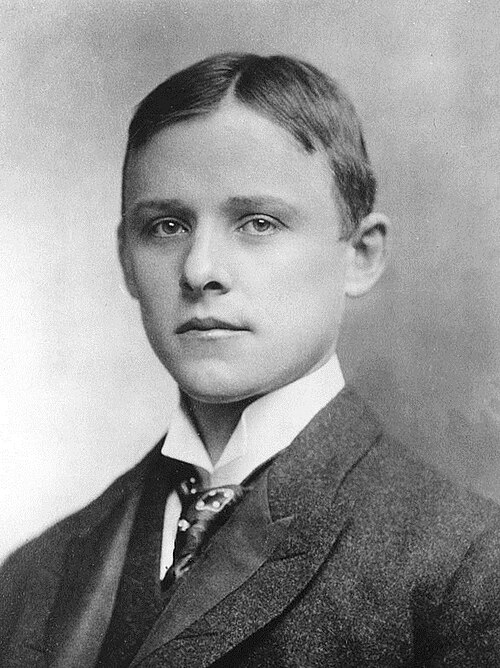
\includegraphics[width=\linewidth]{images/book3/hall.jpg}
\end{minipage}\hspace{0.02\linewidth}%
\begin{minipage}[t]{0.18\linewidth}
\vspace{0pt}
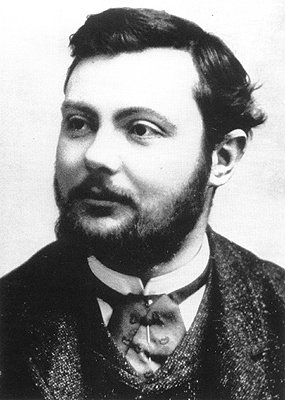
\includegraphics[width=\linewidth]{images/book3/heroult.jpg}
\end{minipage}\hfill
\begin{minipage}[t]{0.58\linewidth}
\vspace{0pt}
En 1886, à vingt-deux ou vingt-trois ans, Charles Martin Hall et
Paul Héroult, de part et d'autre de l'Atlantique, découvrirent indépendamment que l'alumine
se dissout dans la cryolithe fondue et peut y être électrolysée. L'aluminium, jusque-là
un métal précieux obtenu en réduisant son chlorure par le sodium, devint le
moins cher des métaux légers dès que l'électricité put être produite en masse.
(Portraits~: Hall, vers les années 1880, auteur inconnu, domaine public~; Héroult,
domaine public~; Wikimedia Commons.)
\end{minipage}
\end{history}

\paragraph{Le sodium.} Le sodium ne peut pas être déposé à partir de l'eau, qu'il réduit.
On le produit par \omterm{def:b2:batteries-electrolysis:electrolysis}{électrolyse} du chlorure de sodium fondu, dont la température de fusion est
abaissée par un sel ajouté (un \omterm{def:b2:solid-liquid-diagrams:eutectic}{mélange eutectique}, \cref{ch:b2:solid-liquid-diagrams}),
avec du dichlore comme sous-produit. À \qty{1100}{K}, $\Delta_f G^\circ(\ce{NaCl}, \text{l}) =
\qty{-310.7}{kJ/mol}$~: la tension minimale vaut \qty{3.22}{V}.
% ledger: janafG:NaCl.1100

\section{Exercices}

\begin{exercise}[$\star$]\label{exo:b2:batteries-electrolysis:1}
Sur la figure du zinc dans l'acide, lire le \omterm{def:b2:batteries-electrolysis:mixed-potential}{potentiel mixte} et le courant du zinc
seul et du zinc au contact du cuivre (unités du modèle), et dire lequel se dissout
le plus vite.
\end{exercise}

\begin{exercise}[$\star$]\label{exo:b2:batteries-electrolysis:2}
Quelle masse de zinc un courant de \qty{500}{A} dépose-t-il en une heure avec un
\omterm{def:b2:batteries-electrolysis:faradaic-efficiency}{rendement faradique} de 100~\%~?
\end{exercise}

\begin{exercise}[$\star$]\label{exo:b2:batteries-electrolysis:3}
Calculer la tension standard de l'\omterm{def:b2:batteries-electrolysis:battery}{accumulateur} au plomb à partir des \omterm{def:b2:reaction-free-energy:gibbs-energy}{enthalpies libres}
de formation données dans le chapitre, ainsi que le nombre d'éléments d'une
batterie de voiture de \qty{12}{V}.
\end{exercise}

\begin{exercise}[$\star$]\label{exo:b2:batteries-electrolysis:4}
Quelle charge, en ampères-heures, un gramme de lithium peut-il fournir s'il est entièrement
oxydé en \ce{Li+}~?
\end{exercise}

\begin{exercise}[$\star\star$]\label{exo:b2:batteries-electrolysis:5}
Une cuve d'affinage du cuivre est traversée par \qty{200}{A} pendant \qty{24}{h} et dépose
\qty{5.50}{kg} de cuivre. Calculer le \omterm{def:b2:batteries-electrolysis:faradaic-efficiency}{rendement faradique}.
\end{exercise}

\begin{exercise}[$\star\star$]\label{exo:b2:batteries-electrolysis:6}
Une cuve d'\omterm{def:b2:batteries-electrolysis:electrolysis}{électrolyse} du zinc fonctionne sous \qty{3.3}{V} avec un \omterm{def:b2:batteries-electrolysis:faradaic-efficiency}{rendement faradique} de
90~\% (données de l'exercice). Calculer l'énergie électrique par kilogramme de zinc.
\end{exercise}

\begin{exercise}[$\star\star$]\label{exo:b2:batteries-electrolysis:7}
Une pile donne \qty{1.55}{V} sous \qty{0.10}{A} et \qty{1.40}{V} sous \qty{0.60}{A}.
En négligeant les \omterm{def:b2:current-potential-curves:overpotential}{surtensions}, déterminer sa résistance interne et sa
tension à courant nul.
\end{exercise}

\begin{exercise}[$\star\star$]\label{exo:b2:batteries-electrolysis:8}
On \omterm{def:b2:batteries-electrolysis:electrolysis}{électrolyse} de la saumure dans la cellule à membrane. Écrire les réactions aux électrodes,
calculer la tension minimale, et expliquer pourquoi les produits doivent être tenus
séparés.
\end{exercise}

\begin{exercise}[$\star\star$]\label{exo:b2:batteries-electrolysis:9}
Calculer la tension minimale de l'\omterm{def:b2:batteries-electrolysis:electrolysis}{électrolyse} du chlorure de sodium fondu à
\qty{1100}{K} et l'énergie minimale par kilogramme de sodium.
\end{exercise}

\begin{exercise}[$\star\star\star$]\label{exo:b2:batteries-electrolysis:10}
À l'aide des \omterm{def:b2:current-potential-curves:ie-curve}{courbes intensité--potentiel}, expliquer pourquoi on peut déposer du zinc à partir d'un
bain acide sur une cathode de zinc, et prévoir ce qui se passerait sur une cathode de platine au
début du dépôt.
\end{exercise}

\begin{exercise}[$\star\star\star$]\label{exo:b2:batteries-electrolysis:11}
À partir des $\Delta_f G^\circ$ à \qty{1100}{K} et \qty{1300}{K} ($\ce{Al2O3}$~: $-1328.3$ et
$-1262.3$~; $\ce{CO2}$~: $-396.0$ et $-396.2$ \unit{kJ/mol}), calculer la tension
minimale de la cuve Hall--Héroult à \qty{1250}{K}, et la comparer à celle d'une
anode inerte sur laquelle se dégagerait du dioxygène.
\end{exercise}

\begin{exercise}[$\star\star\star$]\label{exo:b2:batteries-electrolysis:12}
On stocke de l'électricité en électrolysant de l'eau sous \qty{1.80}{V} et on la récupère dans une
\omterm{def:b2:batteries-electrolysis:fuel-cell}{pile à combustible} sous \qty{0.70}{V}, toutes deux avec un \omterm{def:b2:batteries-electrolysis:faradaic-efficiency}{rendement faradique} de 100~\%. Calculer le
rendement global de l'aller-retour et expliquer où passe l'énergie.
\end{exercise}

\section{Problème~: une tonne d'aluminium}

\begin{problem}[{Problème du week-end --- la réaction de la cuve Hall--Héroult
et sa tension minimale, la charge et la durée nécessaires pour produire une tonne d'aluminium,
l'énergie consommée, et le carbone brûlé}]
\label{pb:b2:batteries-electrolysis:1}
Données~: \omterm{def:b2:reaction-free-energy:gibbs-energy}{enthalpies libres} de formation JANAF à \qty{1100}{K} et \qty{1300}{K}
(\unit{kJ/mol})~: \ce{Al2O3} $-1328.3$, $-1262.3$~; \ce{CO2} $-396.0$, $-396.2$. Cuve
(données de l'exercice)~: courant \qty{300}{kA}, tension \qty{4.1}{V}, \omterm{def:b2:batteries-electrolysis:faradaic-efficiency}{rendement faradique}
94~\%, bain vers \qty{1250}{K}. Masses molaires (\unit{g/mol})~: Al 26.982, C 12.011,
O 15.999. Chaleur nécessaire pour porter l'aluminium de \qty{298}{K} à l'état liquide à sa température de
fusion~: \qty{28.69}{kJ/mol}.
% ledger: janafG:Al2O3.1100, janafG:Al2O3.1300, janafG:CO2.1100, janafG:CO2.1300, aw:Al, aw:C, aw:O, hT:Al_l.933, const:F

\medskip
\noindent\textbf{Partie I --- La tension minimale.}
\begin{enumerate}
  \item Donner les nombres d'oxydation de l'aluminium, de l'oxygène et du carbone dans les
        réactifs et les produits.
  \item Écrire les demi-équations à la cathode et à l'anode, l'ion oxyde
        \ce{O^2-} étant apporté par le bain fondu.
  \item Écrire la réaction globale et le nombre $n$ d'électrons échangés.
  \item Interpoler les $\Delta_f G^\circ$ de \ce{Al2O3} et de \ce{CO2} à \qty{1250}{K}.
  \item Calculer $\Delta_r G^\circ$ à \qty{1250}{K}.
  \item En déduire la tension minimale.
  \item Calculer la tension minimale avec une anode inerte,
        \ce{2Al2O3 -> 4Al + 3O2}, et expliquer le rôle du carbone.
\end{enumerate}

\medskip
\noindent\textbf{Partie II --- Charge et durée.}
\begin{enumerate}[resume]
  \item Quelle quantité d'aluminium contient une tonne~?
  \item Quelle charge faudrait-il avec un \omterm{def:b2:batteries-electrolysis:faradaic-efficiency}{rendement faradique} de 100~\%~?
  \item Quelle charge passe réellement~?
  \item Combien de temps une cuve met-elle pour produire une tonne~?
  \item Quelle masse d'aluminium une cuve produit-elle par jour~?
  \item Proposer une explication à la perte de 6~\% de la charge.
\end{enumerate}

\medskip
\noindent\textbf{Partie III --- L'énergie.}
\begin{enumerate}[resume]
  \item Calculer l'énergie électrique par tonne.
  \item L'exprimer en \unit{kW.h} par kilogramme.
  \item Calculer l'énergie minimale par kilogramme, sous la tension minimale et avec un
        rendement de 100~\%.
  \item Où passe le reste de l'énergie, et pourquoi n'est-il pas entièrement
        perdu~?
  \item Calculer la puissance électrique d'une cuve.
  \item Calculer la chaleur nécessaire pour refondre un kilogramme de déchets, en
        \unit{kW.h}, et comparer.
  \item Quelle fraction de la tension de fonctionnement représente le minimum thermodynamique~?
\end{enumerate}

\medskip
\noindent\textbf{Partie IV --- Le carbone.}
\begin{enumerate}[resume]
  \item Calculer la masse de carbone brûlée par tonne d'aluminium d'après
        l'équation.
  \item Calculer la masse de dioxyde de carbone libérée par les anodes par tonne.
  \item Les cuves réelles brûlent davantage de carbone. Proposer deux raisons.
  \item Exprimer le \ce{CO2} des anodes par kilogramme d'aluminium.
  \item Que changerait une anode inerte pour la tension et pour le gaz
        dégagé~?
  \item Donner l'énergie électrique par kilogramme d'aluminium.
\end{enumerate}
\end{problem}
